% Generated by Sphinx.
\def\sphinxdocclass{report}
\documentclass[letterpaper,10pt,english]{sphinxmanual}
\usepackage[utf8]{inputenc}
\DeclareUnicodeCharacter{00A0}{\nobreakspace}
\usepackage{cmap}
\usepackage[T1]{fontenc}
\usepackage{babel}
\usepackage{times}
\usepackage[Bjarne]{fncychap}
\usepackage{longtable}
\usepackage{sphinx}
\usepackage{multirow}

\addto\captionsenglish{\renewcommand{\figurename}{Fig. }}
\addto\captionsenglish{\renewcommand{\tablename}{Table }}
\floatname{literal-block}{Listing }



\title{JetChars Documentation}
\date{May 18, 2015}
\release{0.1}
\author{JetChars}
\newcommand{\sphinxlogo}{}
\renewcommand{\releasename}{Release}
\makeindex

\makeatletter
\def\PYG@reset{\let\PYG@it=\relax \let\PYG@bf=\relax%
    \let\PYG@ul=\relax \let\PYG@tc=\relax%
    \let\PYG@bc=\relax \let\PYG@ff=\relax}
\def\PYG@tok#1{\csname PYG@tok@#1\endcsname}
\def\PYG@toks#1+{\ifx\relax#1\empty\else%
    \PYG@tok{#1}\expandafter\PYG@toks\fi}
\def\PYG@do#1{\PYG@bc{\PYG@tc{\PYG@ul{%
    \PYG@it{\PYG@bf{\PYG@ff{#1}}}}}}}
\def\PYG#1#2{\PYG@reset\PYG@toks#1+\relax+\PYG@do{#2}}

\expandafter\def\csname PYG@tok@gd\endcsname{\def\PYG@tc##1{\textcolor[rgb]{0.63,0.00,0.00}{##1}}}
\expandafter\def\csname PYG@tok@gu\endcsname{\let\PYG@bf=\textbf\def\PYG@tc##1{\textcolor[rgb]{0.50,0.00,0.50}{##1}}}
\expandafter\def\csname PYG@tok@gt\endcsname{\def\PYG@tc##1{\textcolor[rgb]{0.00,0.27,0.87}{##1}}}
\expandafter\def\csname PYG@tok@gs\endcsname{\let\PYG@bf=\textbf}
\expandafter\def\csname PYG@tok@gr\endcsname{\def\PYG@tc##1{\textcolor[rgb]{1.00,0.00,0.00}{##1}}}
\expandafter\def\csname PYG@tok@cm\endcsname{\let\PYG@it=\textit\def\PYG@tc##1{\textcolor[rgb]{0.25,0.50,0.56}{##1}}}
\expandafter\def\csname PYG@tok@vg\endcsname{\def\PYG@tc##1{\textcolor[rgb]{0.73,0.38,0.84}{##1}}}
\expandafter\def\csname PYG@tok@m\endcsname{\def\PYG@tc##1{\textcolor[rgb]{0.13,0.50,0.31}{##1}}}
\expandafter\def\csname PYG@tok@mh\endcsname{\def\PYG@tc##1{\textcolor[rgb]{0.13,0.50,0.31}{##1}}}
\expandafter\def\csname PYG@tok@cs\endcsname{\def\PYG@tc##1{\textcolor[rgb]{0.25,0.50,0.56}{##1}}\def\PYG@bc##1{\setlength{\fboxsep}{0pt}\colorbox[rgb]{1.00,0.94,0.94}{\strut ##1}}}
\expandafter\def\csname PYG@tok@ge\endcsname{\let\PYG@it=\textit}
\expandafter\def\csname PYG@tok@vc\endcsname{\def\PYG@tc##1{\textcolor[rgb]{0.73,0.38,0.84}{##1}}}
\expandafter\def\csname PYG@tok@il\endcsname{\def\PYG@tc##1{\textcolor[rgb]{0.13,0.50,0.31}{##1}}}
\expandafter\def\csname PYG@tok@go\endcsname{\def\PYG@tc##1{\textcolor[rgb]{0.20,0.20,0.20}{##1}}}
\expandafter\def\csname PYG@tok@cp\endcsname{\def\PYG@tc##1{\textcolor[rgb]{0.00,0.44,0.13}{##1}}}
\expandafter\def\csname PYG@tok@gi\endcsname{\def\PYG@tc##1{\textcolor[rgb]{0.00,0.63,0.00}{##1}}}
\expandafter\def\csname PYG@tok@gh\endcsname{\let\PYG@bf=\textbf\def\PYG@tc##1{\textcolor[rgb]{0.00,0.00,0.50}{##1}}}
\expandafter\def\csname PYG@tok@ni\endcsname{\let\PYG@bf=\textbf\def\PYG@tc##1{\textcolor[rgb]{0.84,0.33,0.22}{##1}}}
\expandafter\def\csname PYG@tok@nl\endcsname{\let\PYG@bf=\textbf\def\PYG@tc##1{\textcolor[rgb]{0.00,0.13,0.44}{##1}}}
\expandafter\def\csname PYG@tok@nn\endcsname{\let\PYG@bf=\textbf\def\PYG@tc##1{\textcolor[rgb]{0.05,0.52,0.71}{##1}}}
\expandafter\def\csname PYG@tok@no\endcsname{\def\PYG@tc##1{\textcolor[rgb]{0.38,0.68,0.84}{##1}}}
\expandafter\def\csname PYG@tok@na\endcsname{\def\PYG@tc##1{\textcolor[rgb]{0.25,0.44,0.63}{##1}}}
\expandafter\def\csname PYG@tok@nb\endcsname{\def\PYG@tc##1{\textcolor[rgb]{0.00,0.44,0.13}{##1}}}
\expandafter\def\csname PYG@tok@nc\endcsname{\let\PYG@bf=\textbf\def\PYG@tc##1{\textcolor[rgb]{0.05,0.52,0.71}{##1}}}
\expandafter\def\csname PYG@tok@nd\endcsname{\let\PYG@bf=\textbf\def\PYG@tc##1{\textcolor[rgb]{0.33,0.33,0.33}{##1}}}
\expandafter\def\csname PYG@tok@ne\endcsname{\def\PYG@tc##1{\textcolor[rgb]{0.00,0.44,0.13}{##1}}}
\expandafter\def\csname PYG@tok@nf\endcsname{\def\PYG@tc##1{\textcolor[rgb]{0.02,0.16,0.49}{##1}}}
\expandafter\def\csname PYG@tok@si\endcsname{\let\PYG@it=\textit\def\PYG@tc##1{\textcolor[rgb]{0.44,0.63,0.82}{##1}}}
\expandafter\def\csname PYG@tok@s2\endcsname{\def\PYG@tc##1{\textcolor[rgb]{0.25,0.44,0.63}{##1}}}
\expandafter\def\csname PYG@tok@vi\endcsname{\def\PYG@tc##1{\textcolor[rgb]{0.73,0.38,0.84}{##1}}}
\expandafter\def\csname PYG@tok@nt\endcsname{\let\PYG@bf=\textbf\def\PYG@tc##1{\textcolor[rgb]{0.02,0.16,0.45}{##1}}}
\expandafter\def\csname PYG@tok@nv\endcsname{\def\PYG@tc##1{\textcolor[rgb]{0.73,0.38,0.84}{##1}}}
\expandafter\def\csname PYG@tok@s1\endcsname{\def\PYG@tc##1{\textcolor[rgb]{0.25,0.44,0.63}{##1}}}
\expandafter\def\csname PYG@tok@gp\endcsname{\let\PYG@bf=\textbf\def\PYG@tc##1{\textcolor[rgb]{0.78,0.36,0.04}{##1}}}
\expandafter\def\csname PYG@tok@sh\endcsname{\def\PYG@tc##1{\textcolor[rgb]{0.25,0.44,0.63}{##1}}}
\expandafter\def\csname PYG@tok@ow\endcsname{\let\PYG@bf=\textbf\def\PYG@tc##1{\textcolor[rgb]{0.00,0.44,0.13}{##1}}}
\expandafter\def\csname PYG@tok@sx\endcsname{\def\PYG@tc##1{\textcolor[rgb]{0.78,0.36,0.04}{##1}}}
\expandafter\def\csname PYG@tok@bp\endcsname{\def\PYG@tc##1{\textcolor[rgb]{0.00,0.44,0.13}{##1}}}
\expandafter\def\csname PYG@tok@c1\endcsname{\let\PYG@it=\textit\def\PYG@tc##1{\textcolor[rgb]{0.25,0.50,0.56}{##1}}}
\expandafter\def\csname PYG@tok@kc\endcsname{\let\PYG@bf=\textbf\def\PYG@tc##1{\textcolor[rgb]{0.00,0.44,0.13}{##1}}}
\expandafter\def\csname PYG@tok@c\endcsname{\let\PYG@it=\textit\def\PYG@tc##1{\textcolor[rgb]{0.25,0.50,0.56}{##1}}}
\expandafter\def\csname PYG@tok@mf\endcsname{\def\PYG@tc##1{\textcolor[rgb]{0.13,0.50,0.31}{##1}}}
\expandafter\def\csname PYG@tok@err\endcsname{\def\PYG@bc##1{\setlength{\fboxsep}{0pt}\fcolorbox[rgb]{1.00,0.00,0.00}{1,1,1}{\strut ##1}}}
\expandafter\def\csname PYG@tok@mb\endcsname{\def\PYG@tc##1{\textcolor[rgb]{0.13,0.50,0.31}{##1}}}
\expandafter\def\csname PYG@tok@ss\endcsname{\def\PYG@tc##1{\textcolor[rgb]{0.32,0.47,0.09}{##1}}}
\expandafter\def\csname PYG@tok@sr\endcsname{\def\PYG@tc##1{\textcolor[rgb]{0.14,0.33,0.53}{##1}}}
\expandafter\def\csname PYG@tok@mo\endcsname{\def\PYG@tc##1{\textcolor[rgb]{0.13,0.50,0.31}{##1}}}
\expandafter\def\csname PYG@tok@kd\endcsname{\let\PYG@bf=\textbf\def\PYG@tc##1{\textcolor[rgb]{0.00,0.44,0.13}{##1}}}
\expandafter\def\csname PYG@tok@mi\endcsname{\def\PYG@tc##1{\textcolor[rgb]{0.13,0.50,0.31}{##1}}}
\expandafter\def\csname PYG@tok@kn\endcsname{\let\PYG@bf=\textbf\def\PYG@tc##1{\textcolor[rgb]{0.00,0.44,0.13}{##1}}}
\expandafter\def\csname PYG@tok@o\endcsname{\def\PYG@tc##1{\textcolor[rgb]{0.40,0.40,0.40}{##1}}}
\expandafter\def\csname PYG@tok@kr\endcsname{\let\PYG@bf=\textbf\def\PYG@tc##1{\textcolor[rgb]{0.00,0.44,0.13}{##1}}}
\expandafter\def\csname PYG@tok@s\endcsname{\def\PYG@tc##1{\textcolor[rgb]{0.25,0.44,0.63}{##1}}}
\expandafter\def\csname PYG@tok@kp\endcsname{\def\PYG@tc##1{\textcolor[rgb]{0.00,0.44,0.13}{##1}}}
\expandafter\def\csname PYG@tok@w\endcsname{\def\PYG@tc##1{\textcolor[rgb]{0.73,0.73,0.73}{##1}}}
\expandafter\def\csname PYG@tok@kt\endcsname{\def\PYG@tc##1{\textcolor[rgb]{0.56,0.13,0.00}{##1}}}
\expandafter\def\csname PYG@tok@sc\endcsname{\def\PYG@tc##1{\textcolor[rgb]{0.25,0.44,0.63}{##1}}}
\expandafter\def\csname PYG@tok@sb\endcsname{\def\PYG@tc##1{\textcolor[rgb]{0.25,0.44,0.63}{##1}}}
\expandafter\def\csname PYG@tok@k\endcsname{\let\PYG@bf=\textbf\def\PYG@tc##1{\textcolor[rgb]{0.00,0.44,0.13}{##1}}}
\expandafter\def\csname PYG@tok@se\endcsname{\let\PYG@bf=\textbf\def\PYG@tc##1{\textcolor[rgb]{0.25,0.44,0.63}{##1}}}
\expandafter\def\csname PYG@tok@sd\endcsname{\let\PYG@it=\textit\def\PYG@tc##1{\textcolor[rgb]{0.25,0.44,0.63}{##1}}}

\def\PYGZbs{\char`\\}
\def\PYGZus{\char`\_}
\def\PYGZob{\char`\{}
\def\PYGZcb{\char`\}}
\def\PYGZca{\char`\^}
\def\PYGZam{\char`\&}
\def\PYGZlt{\char`\<}
\def\PYGZgt{\char`\>}
\def\PYGZsh{\char`\#}
\def\PYGZpc{\char`\%}
\def\PYGZdl{\char`\$}
\def\PYGZhy{\char`\-}
\def\PYGZsq{\char`\'}
\def\PYGZdq{\char`\"}
\def\PYGZti{\char`\~}
% for compatibility with earlier versions
\def\PYGZat{@}
\def\PYGZlb{[}
\def\PYGZrb{]}
\makeatother

\renewcommand\PYGZsq{\textquotesingle}

\begin{document}

\maketitle
\tableofcontents
\phantomsection\label{index::doc}



\chapter{DevStack Hacking}
\label{index:welcome-to-jetchars-s-documentation}\label{index:devstack-hacking}

\section{Enable DVR with DevStack}
\label{docs/enable_dvr_with_devstack/index:enable-dvr-with-devstack}\label{docs/enable_dvr_with_devstack/index::doc}
DVR is short for distributed virtual router, with this feature enabled packets flow with floating IP will no longer send to network node. It helps to alleviate network node's pressure greatly when large amount of north-south data flow occurs. \footnote{
\href{https://wiki.openstack.org/wiki/Neutron/DVR/HowTo}{https://wiki.openstack.org/wiki/Neutron/DVR/HowTo}
}


\subsection{Brief Intro}
\label{docs/enable_dvr_with_devstack/index:brief-intro}
In order to enable distributed router on each compute-node, Neutron-metadata-agent and Neutron-L3-agent are both needed. So we need to add \textbf{q-meta} and \textbf{q-l3} as well as \emph{q-agt} on each computer node's \code{local.conf} file.

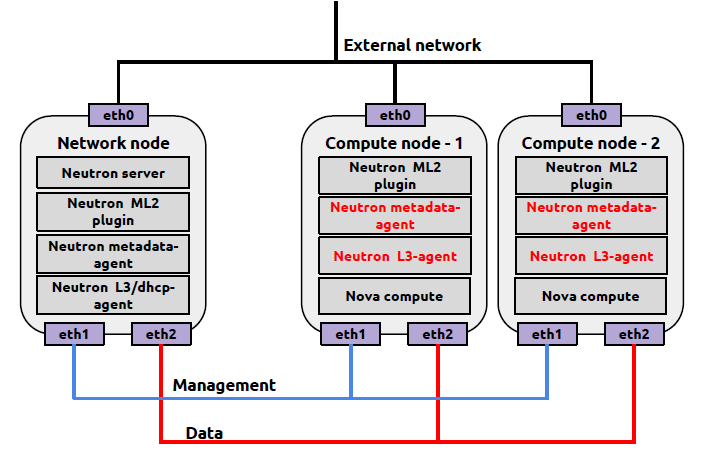
\includegraphics{image1.png}

\begin{notice}{warning}{Warning:}
Currently devstack doesn't support deploying DVR on GRE tunnel \footnote{
\href{https://blueprints.launchpad.net/neutron/+spec/neutron-ovs-dvr}{https://blueprints.launchpad.net/neutron/+spec/neutron-ovs-dvr}
} , and tunnel type has been hard coded to vxlan mode, the following is a part of devstack's code \code{lib/neutron\_plugins/ml2}:
\end{notice}

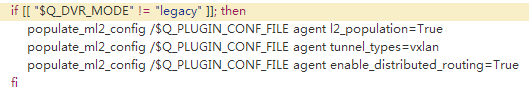
\includegraphics{image2.png}

With DVR, floating IPs can be accessed directly from each compute node, but SNAT still need to be centralized to network node.

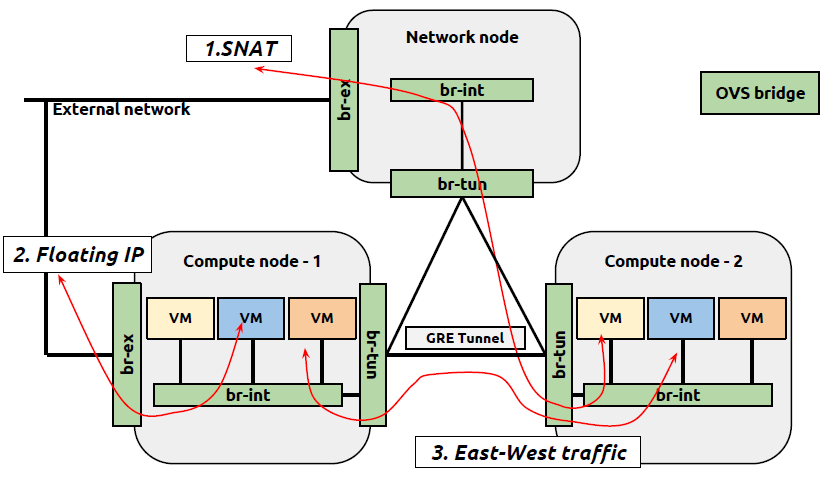
\includegraphics{image3.png}


\subsection{Configure Network Node}
\label{docs/enable_dvr_with_devstack/index:configure-network-node}
Here's the neutron configuration part of \code{local.conf} on network node.

\begin{Verbatim}[commandchars=\\\{\},numbers=left,firstnumber=1,stepnumber=1]
\PYG{c}{\PYGZsh{} Neutron\PYGZhy{}vxlan\PYGZhy{}tunnel\PYGZhy{}DVR}
\PYG{c}{\PYGZsh{}\PYGZsh{}\PYGZsh{}\PYGZsh{}\PYGZsh{}\PYGZsh{}\PYGZsh{}\PYGZsh{}\PYGZsh{}\PYGZsh{}\PYGZsh{}\PYGZsh{}\PYGZsh{}\PYGZsh{}\PYGZsh{}\PYGZsh{}\PYGZsh{}\PYGZsh{}\PYGZsh{}\PYGZsh{}\PYGZsh{}\PYGZsh{}\PYGZsh{}\PYGZsh{}\PYGZsh{}\PYGZsh{}}
ENABLED\PYGZus{}SERVICES+\PYG{o}{=},q\PYGZhy{}svc,q\PYGZhy{}agt,q\PYGZhy{}dhcp,q\PYGZhy{}l3,q\PYGZhy{}meta,neutron
\PYG{n+nv}{Q\PYGZus{}FLOATING\PYGZus{}ALLOCATION\PYGZus{}POOL}\PYG{o}{=}\PYG{n+nv}{start}\PYG{o}{=}192.168.137.166,end\PYG{o}{=}192.168.137.253
\PYG{n+nv}{Q\PYGZus{}ROUTER\PYGZus{}NAME}\PYG{o}{=}default\PYGZus{}router
\PYG{n+nv}{PUBLIC\PYGZus{}NETWORK\PYGZus{}GATEWAY}\PYG{o}{=}192.168.137.254
\PYG{n+nv}{FLOATING\PYGZus{}RANGE}\PYG{o}{=}192.168.0.0/16

\PYG{n+nv}{FIXED\PYGZus{}RANGE}\PYG{o}{=}10.1.1.0/24
\PYG{n+nv}{FIXED\PYGZus{}NETWORK\PYGZus{}SIZE}\PYG{o}{=}256
\PYG{n+nv}{NETWORK\PYGZus{}GATEWAY}\PYG{o}{=}10.1.1.1

\PYG{n+nv}{Q\PYGZus{}PLUGIN}\PYG{o}{=}ml2
\PYG{n+nv}{Q\PYGZus{}ML2\PYGZus{}TENANT\PYGZus{}NETWORK\PYGZus{}TYPE}\PYG{o}{=}vxlan
\PYG{n+nv}{TUNNEL\PYGZus{}ENDPOINT\PYGZus{}IP}\PYG{o}{=}192.168.1.37
\PYG{n+nv}{Q\PYGZus{}DVR\PYGZus{}MODE}\PYG{o}{=}dvr\PYGZus{}snat
\PYG{n+nv}{Q\PYGZus{}SERVICE\PYGZus{}PLUGIN\PYGZus{}CLASSES}\PYG{o}{=}neutron.services.l3\PYGZus{}router.l3\PYGZus{}router\PYGZus{}plugin.L3RouterPlugin
\PYG{n+nv}{Q\PYGZus{}ML2\PYGZus{}PLUGIN\PYGZus{}MECHANISM\PYGZus{}DRIVERS}\PYG{o}{=}openvswitch,linuxbridge,l2population
\end{Verbatim}

\begin{notice}{note}{Note:}
DVR mode can be \textbf{dvr\_snat} , \textbf{dvr} or \textbf{legacy}. \emph{Legacy} is Q\_DVR\_MODE `s default value, \emph{dvr\_snat} is for network node which enables snat router, and \emph{dvr} mode is for compute node.
\end{notice}

\textbf{L2population} is needed by DVR. The L2 Population driver enables broadcast, multicast, and unicast traffic to scale out on large overlay networks. This traffic is sent to the relevant agent via encapsulation as a targeted unicast. \footnote{
\href{https://wiki.openstack.org/wiki/Neutron/DVR\_L2\_Agent}{https://wiki.openstack.org/wiki/Neutron/DVR\_L2\_Agent}
}

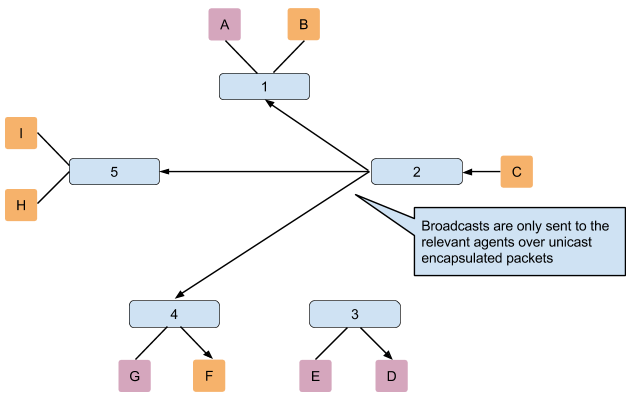
\includegraphics{image4.png}

After Installation you might see 3 bridges and 4 namespaces on network node.

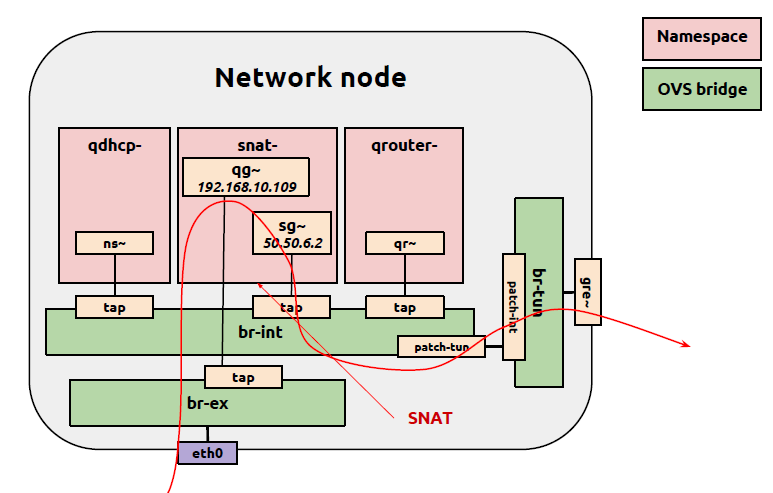
\includegraphics{image5.png}

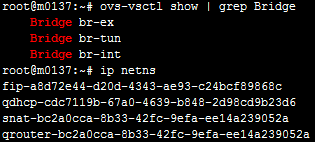
\includegraphics{image6.png}

Namespace fip* is for floating IP accessing. qdhcp* is for allocating IP addresses. snat* is for SNAT function. qrouter* only serves VM in current host.


\subsection{Configure Compute Node}
\label{docs/enable_dvr_with_devstack/index:configure-compute-node}
The following is the neutron configuration part of \code{local.conf} on compute node

\begin{Verbatim}[commandchars=\\\{\},numbers=left,firstnumber=1,stepnumber=1]
\PYG{c}{\PYGZsh{} Neutron\PYGZhy{}vxlan\PYGZhy{}tunnel\PYGZhy{}DVR}
\PYG{c}{\PYGZsh{}\PYGZsh{}\PYGZsh{}\PYGZsh{}\PYGZsh{}\PYGZsh{}\PYGZsh{}\PYGZsh{}\PYGZsh{}\PYGZsh{}\PYGZsh{}\PYGZsh{}\PYGZsh{}\PYGZsh{}\PYGZsh{}\PYGZsh{}\PYGZsh{}\PYGZsh{}\PYGZsh{}\PYGZsh{}\PYGZsh{}\PYGZsh{}\PYGZsh{}\PYGZsh{}\PYGZsh{}\PYGZsh{}}
ENABLED\PYGZus{}SERVICES+\PYG{o}{=} q\PYGZhy{}agt,q\PYGZhy{}l3,q\PYGZhy{}meta, neutron
\PYG{n+nv}{Q\PYGZus{}PLUGIN}\PYG{o}{=}ml2
\PYG{n+nv}{Q\PYGZus{}ML2\PYGZus{}TENANT\PYGZus{}NETWORK\PYGZus{}TYPE}\PYG{o}{=}vxlan
\PYG{n+nv}{TUNNEL\PYGZus{}ENDPOINT\PYGZus{}IP}\PYG{o}{=}192.168.1.34
\PYG{n+nv}{Q\PYGZus{}DVR\PYGZus{}MODE}\PYG{o}{=}dvr
\PYG{n+nv}{Q\PYGZus{}SERVICE\PYGZus{}PLUGIN\PYGZus{}CLASSES}\PYG{o}{=}neutron.services.l3\PYGZus{}router.l3\PYGZus{}router\PYGZus{}plugin.L3RouterPlugin
\PYG{n+nv}{Q\PYGZus{}ML2\PYGZus{}PLUGIN\PYGZus{}MECHANISM\PYGZus{}DRIVERS}\PYG{o}{=}openvswitch,linuxbridge,l2population
\end{Verbatim}

After installation you might see 3 bridges and 2 namespaces.

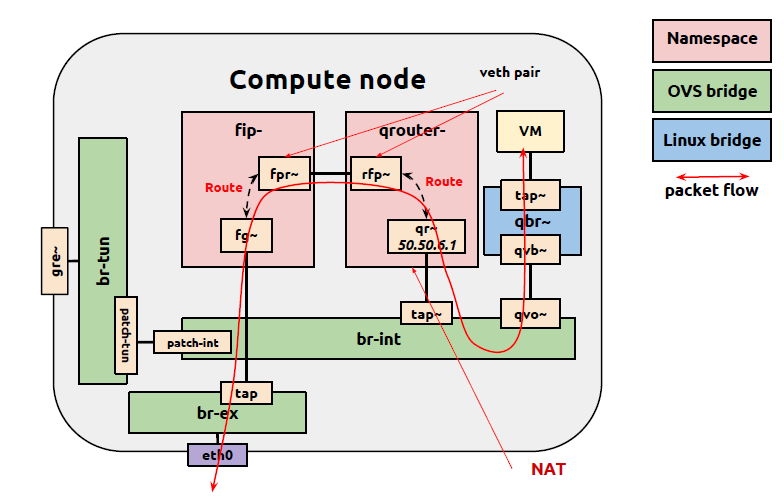
\includegraphics{image7.png}

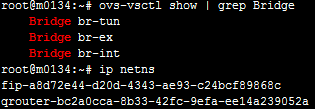
\includegraphics{image8.png}

fip* and qrouter* did the same job as two virtual devices on network node.
We still need to do some configurations manually.
\begin{enumerate}
\item {} 
Add an free physical device(NIC) to br-ex

\end{enumerate}

\begin{Verbatim}[commandchars=\\\{\}]
\PYG{n+nv}{\PYGZdl{} }sudo ovs\PYGZhy{}vsctl add\PYGZhy{}port br\PYGZhy{}ex eth1
\end{Verbatim}
\begin{enumerate}
\setcounter{enumi}{1}
\item {} 
Allocate an IP for br-ex as a gateway

\end{enumerate}

\begin{Verbatim}[commandchars=\\\{\}]
\PYG{n+nv}{\PYGZdl{} }sudo ifconfig br\PYGZhy{}ex 192.168.137.253
\end{Verbatim}
\begin{enumerate}
\setcounter{enumi}{2}
\item {} 
Add a route to floating network via fip*

\end{enumerate}

Before we adding this route, we need to know fip's IP address.

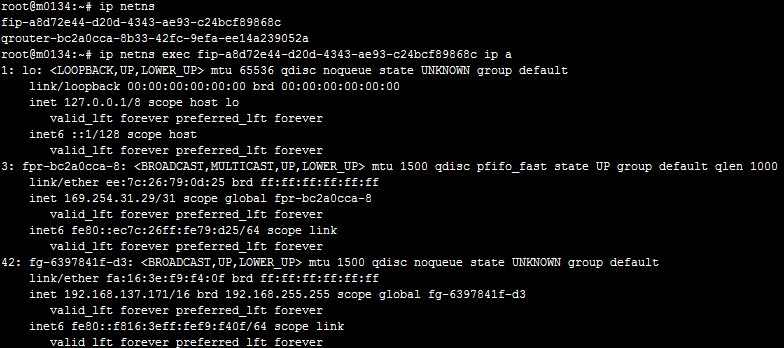
\includegraphics{image9.png}

We use the IP on fg* .

\begin{Verbatim}[commandchars=\\\{\}]
\PYG{n+nv}{\PYGZdl{} }sudo ip route add 192.168.0.0/16 via 192.168.137.171
\end{Verbatim}


\subsection{References}
\label{docs/enable_dvr_with_devstack/index:references}

\chapter{OpenStack Customization}
\label{index:openstack-customization}

\section{KVM Optimization}
\label{docs/kvm_optimization/index:kvm-optimization}\label{docs/kvm_optimization/index::doc}

\subsection{Disk Optimization}
\label{docs/kvm_optimization/index:disk-optimization}

\subsubsection{Asynchronous IO}
\label{docs/kvm_optimization/index:asynchronous-io}

\subsubsection{Disk Cache Mode}
\label{docs/kvm_optimization/index:disk-cache-mode}

\subsection{Memory Optimization}
\label{docs/kvm_optimization/index:memory-optimization}

\subsubsection{Transparent HugePage}
\label{docs/kvm_optimization/index:transparent-hugepage}

\subsection{Network Optimization}
\label{docs/kvm_optimization/index:network-optimization}

\subsubsection{MTU Size}
\label{docs/kvm_optimization/index:mtu-size}

\chapter{Hadoop Tuning}
\label{index:hadoop-tuning}

\section{HiBench - The Hadoop BenchMark Suit}
\label{docs/hibench_intro/index:hibench-the-hadoop-benchmark-suit}\label{docs/hibench_intro/index::doc}
Most of my hadoop tuning data derived with this benchmark tool.


\subsection{What is HiBench? \footnote{
https://github.com/intel-hadoop/Hibench
}}
\label{docs/hibench_intro/index:what-is-hibench}
This benchmark suite contains 10 typical Hadoop workloads (including micro benchmarks, HDFS benchmarks, web search benchmarks, machine learning benchmarks, and data analytics benchmarks). \footnote{
\href{http://ieeexplore.ieee.org/xpl/articleDetails.jsp?reload=true\&arnumber=5452747}{http://ieeexplore.ieee.org/xpl/articleDetails.jsp?reload=true\&arnumber=5452747}
}

Advantages:
\begin{itemize}
\item {} 
Realistic and comprehensive

\item {} 
Quantitive characteriztion of different workload

\item {} 
Evaluation of different deployment

\end{itemize}


\subsection{BenchMark Types}
\label{docs/hibench_intro/index:benchmark-types}
HiBench Contains 5 different types of benchmark.
\begin{enumerate}
\item {} 
micro benchmarks: \code{Sort} \code{WordCount} \code{TeraSort}

\item {} 
HDFS benchmarks: \code{enhanced DFSIO} \code{Sleep}

\item {} 
web search benchmarks: \code{Nutching indexing} \code{PageRank}

\item {} 
machine learning benchmarks: \code{Bayes Classification} \code{K-means} \code{Clustering}

\item {} 
data analytics benchmarks: \code{Hive} \code{Query} \code{Benchmark}

\end{enumerate}


\subsection{Configuration \& Running scripts}
\label{docs/hibench_intro/index:configuration-running-scripts}
Global enviroment variable in \code{bin/hibench-config.sh}

Each workload can run separately:
\begin{itemize}
\item {} 
\code{conf/configure.sh}  Configuration file contains all parameters such as data size and test options.

\item {} 
\code{bin/prepare*.sh}    Generate or copy each workload's prepare data into HDFS.

\item {} 
\code{bin/run*.sh}        Execute the workload

\end{itemize}


\subsection{Default Configurations}
\label{docs/hibench_intro/index:default-configurations}
Default configurations' data size normally very small.(Release version: 3.0)


\subsubsection{DFSIOE}
\label{docs/hibench_intro/index:dfsioe}
\begin{Verbatim}[commandchars=\\\{\},numbers=left,firstnumber=1,stepnumber=1]
\PYG{c}{\PYGZsh{}\PYGZsh{} paths}
\PYG{n+nv}{INPUT\PYGZus{}HDFS}\PYG{o}{=}\PYG{l+s+si}{\PYGZdl{}\PYGZob{}}\PYG{n+nv}{DATA\PYGZus{}HDFS}\PYG{l+s+si}{\PYGZcb{}}/benchmarks/TestDFSIO\PYGZhy{}Enh

\PYG{n+nb}{export }\PYG{n+nv}{HADOOP\PYGZus{}OPTS}\PYG{o}{=}\PYG{l+s+s2}{\PYGZdq{}}\PYG{n+nv}{\PYGZdl{}HADOOP\PYGZus{}OPTS}\PYG{l+s+s2}{ \PYGZhy{}Dtest.build.data=}\PYG{l+s+si}{\PYGZdl{}\PYGZob{}}\PYG{n+nv}{INPUT\PYGZus{}HDFS}\PYG{l+s+si}{\PYGZcb{}}\PYG{l+s+s2}{\PYGZdq{}}
\PYG{n+nv}{MAP\PYGZus{}JAVA\PYGZus{}OPTS}\PYG{o}{=}\PYG{l+s+sb}{{}`}cat \PYG{n+nv}{\PYGZdl{}HADOOP\PYGZus{}CONF\PYGZus{}DIR}/mapred\PYGZhy{}site.xml \PYG{p}{\textbar{}} grep \PYG{l+s+s2}{\PYGZdq{}mapreduce.map.java.opts\PYGZdq{}} \PYG{p}{\textbar{}} awk \PYGZhy{}F\PYG{l+s+se}{\PYGZbs{}\PYGZlt{}} \PYG{l+s+s1}{\PYGZsq{}\PYGZob{}print \PYGZdl{}5\PYGZcb{}\PYGZsq{}} \PYG{p}{\textbar{}} awk \PYGZhy{}F\PYG{l+s+se}{\PYGZbs{}\PYGZgt{}} \PYG{l+s+s1}{\PYGZsq{}\PYGZob{}print \PYGZdl{}NF\PYGZcb{}\PYGZsq{}}\PYG{l+s+sb}{{}`}
\PYG{n+nv}{RED\PYGZus{}JAVA\PYGZus{}OPTS}\PYG{o}{=}\PYG{l+s+sb}{{}`}cat \PYG{n+nv}{\PYGZdl{}HADOOP\PYGZus{}CONF\PYGZus{}DIR}/mapred\PYGZhy{}site.xml \PYG{p}{\textbar{}} grep \PYG{l+s+s2}{\PYGZdq{}mapreduce.reduce.java.opts\PYGZdq{}} \PYG{p}{\textbar{}} awk \PYGZhy{}F\PYG{l+s+se}{\PYGZbs{}\PYGZlt{}} \PYG{l+s+s1}{\PYGZsq{}\PYGZob{}print \PYGZdl{}5\PYGZcb{}\PYGZsq{}} \PYG{p}{\textbar{}} awk \PYGZhy{}F\PYG{l+s+se}{\PYGZbs{}\PYGZgt{}} \PYG{l+s+s1}{\PYGZsq{}\PYGZob{}print \PYGZdl{}NF\PYGZcb{}\PYGZsq{}}\PYG{l+s+sb}{{}`}

\PYG{c}{\PYGZsh{} dfsioe\PYGZhy{}read}
\PYG{n+nv}{RD\PYGZus{}NUM\PYGZus{}OF\PYGZus{}FILES}\PYG{o}{=}256
\PYG{n+nv}{RD\PYGZus{}FILE\PYGZus{}SIZE}\PYG{o}{=}\PYG{l+m}{200} \PYG{c}{\PYGZsh{}2000}

\PYG{c}{\PYGZsh{} dfsioe\PYGZhy{}write}
\PYG{n+nv}{WT\PYGZus{}NUM\PYGZus{}OF\PYGZus{}FILES}\PYG{o}{=}256
\PYG{n+nv}{WT\PYGZus{}FILE\PYGZus{}SIZE}\PYG{o}{=}\PYG{l+m}{100} \PYG{c}{\PYGZsh{}1000}
\end{Verbatim}


\subsubsection{Sort}
\label{docs/hibench_intro/index:sort}
\begin{Verbatim}[commandchars=\\\{\},numbers=left,firstnumber=1,stepnumber=1]
\PYG{c}{\PYGZsh{} compress}
\PYG{n+nv}{COMPRESS}\PYG{o}{=}\PYG{n+nv}{\PYGZdl{}COMPRESS\PYGZus{}GLOBAL}
\PYG{n+nv}{COMPRESS\PYGZus{}CODEC}\PYG{o}{=}\PYG{n+nv}{\PYGZdl{}COMPRESS\PYGZus{}CODEC\PYGZus{}GLOBAL}

\PYG{c}{\PYGZsh{} paths}
\PYG{n+nv}{INPUT\PYGZus{}HDFS}\PYG{o}{=}\PYG{l+s+si}{\PYGZdl{}\PYGZob{}}\PYG{n+nv}{DATA\PYGZus{}HDFS}\PYG{l+s+si}{\PYGZcb{}}/Sort/Input
\PYG{n+nv}{OUTPUT\PYGZus{}HDFS}\PYG{o}{=}\PYG{l+s+si}{\PYGZdl{}\PYGZob{}}\PYG{n+nv}{DATA\PYGZus{}HDFS}\PYG{l+s+si}{\PYGZcb{}}/Sort/Output

\PYG{k}{if} \PYG{o}{[} \PYG{n+nv}{\PYGZdl{}COMPRESS} \PYGZhy{}eq \PYG{l+m}{1} \PYG{o}{]}\PYG{p}{;} \PYG{k}{then}
    \PYG{n+nv}{INPUT\PYGZus{}HDFS}\PYG{o}{=}\PYG{l+s+si}{\PYGZdl{}\PYGZob{}}\PYG{n+nv}{INPUT\PYGZus{}HDFS}\PYG{l+s+si}{\PYGZcb{}}\PYGZhy{}comp
    \PYG{n+nv}{OUTPUT\PYGZus{}HDFS}\PYG{o}{=}\PYG{l+s+si}{\PYGZdl{}\PYGZob{}}\PYG{n+nv}{OUTPUT\PYGZus{}HDFS}\PYG{l+s+si}{\PYGZcb{}}\PYGZhy{}comp
\PYG{k}{fi}

\PYG{c}{\PYGZsh{} for prepare (per node) \PYGZhy{} 24G/node}
\PYG{c}{\PYGZsh{}DATASIZE=24000000000}
\PYG{n+nv}{DATASIZE}\PYG{o}{=}2400000000
\PYG{n+nv}{NUM\PYGZus{}MAPS}\PYG{o}{=}16

\PYG{c}{\PYGZsh{} for running (in total)}
\PYG{n+nv}{NUM\PYGZus{}REDS}\PYG{o}{=}48
\end{Verbatim}


\subsubsection{WordCount}
\label{docs/hibench_intro/index:wordcount}
\begin{Verbatim}[commandchars=\\\{\},numbers=left,firstnumber=1,stepnumber=1]
\PYG{c}{\PYGZsh{} compress}
\PYG{c}{\PYGZsh{} for best performance set COMPRESS=1 for MR1 and COMPRESS=0 for MR2 (for WordCount)}
\PYG{n+nv}{COMPRESS}\PYG{o}{=}\PYG{n+nv}{\PYGZdl{}COMPRESS\PYGZus{}GLOBAL}
\PYG{n+nv}{COMPRESS\PYGZus{}CODEC}\PYG{o}{=}\PYG{n+nv}{\PYGZdl{}COMPRESS\PYGZus{}CODEC\PYGZus{}GLOBAL}

\PYG{c}{\PYGZsh{} paths}
\PYG{n+nv}{INPUT\PYGZus{}HDFS}\PYG{o}{=}\PYG{l+s+si}{\PYGZdl{}\PYGZob{}}\PYG{n+nv}{DATA\PYGZus{}HDFS}\PYG{l+s+si}{\PYGZcb{}}/Wordcount/Input
\PYG{n+nv}{OUTPUT\PYGZus{}HDFS}\PYG{o}{=}\PYG{l+s+si}{\PYGZdl{}\PYGZob{}}\PYG{n+nv}{DATA\PYGZus{}HDFS}\PYG{l+s+si}{\PYGZcb{}}/Wordcount/Output

\PYG{k}{if} \PYG{o}{[} \PYG{n+nv}{\PYGZdl{}COMPRESS} \PYGZhy{}eq \PYG{l+m}{1} \PYG{o}{]}\PYG{p}{;} \PYG{k}{then}
    \PYG{n+nv}{INPUT\PYGZus{}HDFS}\PYG{o}{=}\PYG{l+s+si}{\PYGZdl{}\PYGZob{}}\PYG{n+nv}{INPUT\PYGZus{}HDFS}\PYG{l+s+si}{\PYGZcb{}}\PYGZhy{}comp
    \PYG{n+nv}{OUTPUT\PYGZus{}HDFS}\PYG{o}{=}\PYG{l+s+si}{\PYGZdl{}\PYGZob{}}\PYG{n+nv}{OUTPUT\PYGZus{}HDFS}\PYG{l+s+si}{\PYGZcb{}}\PYGZhy{}comp
\PYG{k}{fi}

\PYG{c}{\PYGZsh{} for preparation (per node) \PYGZhy{} 32G}
\PYG{c}{\PYGZsh{}DATASIZE=32000000000}
\PYG{n+nv}{DATASIZE}\PYG{o}{=}3200000000
\PYG{n+nv}{NUM\PYGZus{}MAPS}\PYG{o}{=}16

\PYG{c}{\PYGZsh{} for running (in total)}
\PYG{n+nv}{NUM\PYGZus{}REDS}\PYG{o}{=}48
\end{Verbatim}


\subsubsection{k-means}
\label{docs/hibench_intro/index:k-means}
\begin{Verbatim}[commandchars=\\\{\},numbers=left,firstnumber=1,stepnumber=1]
\PYG{c}{\PYGZsh{} compress}
\PYG{n+nv}{COMPRESS}\PYG{o}{=}\PYG{n+nv}{\PYGZdl{}COMPRESS\PYGZus{}GLOBAL}
\PYG{n+nv}{COMPRESS\PYGZus{}CODEC}\PYG{o}{=}\PYG{n+nv}{\PYGZdl{}COMPRESS\PYGZus{}CODEC\PYGZus{}GLOBAL}

\PYG{c}{\PYGZsh{} paths}
\PYG{n+nv}{INPUT\PYGZus{}HDFS}\PYG{o}{=}\PYG{l+s+si}{\PYGZdl{}\PYGZob{}}\PYG{n+nv}{DATA\PYGZus{}HDFS}\PYG{l+s+si}{\PYGZcb{}}/KMeans/Input
\PYG{n+nv}{OUTPUT\PYGZus{}HDFS}\PYG{o}{=}\PYG{l+s+si}{\PYGZdl{}\PYGZob{}}\PYG{n+nv}{DATA\PYGZus{}HDFS}\PYG{l+s+si}{\PYGZcb{}}/KMeans/Output
\PYG{k}{if} \PYG{o}{[} \PYG{n+nv}{\PYGZdl{}COMPRESS} \PYGZhy{}eq \PYG{l+m}{1} \PYG{o}{]}\PYG{p}{;} \PYG{k}{then}
    \PYG{n+nv}{INPUT\PYGZus{}HDFS}\PYG{o}{=}\PYG{l+s+si}{\PYGZdl{}\PYGZob{}}\PYG{n+nv}{INPUT\PYGZus{}HDFS}\PYG{l+s+si}{\PYGZcb{}}\PYGZhy{}comp
    \PYG{n+nv}{OUTPUT\PYGZus{}HDFS}\PYG{o}{=}\PYG{l+s+si}{\PYGZdl{}\PYGZob{}}\PYG{n+nv}{OUTPUT\PYGZus{}HDFS}\PYG{l+s+si}{\PYGZcb{}}\PYGZhy{}comp
\PYG{k}{fi}
\PYG{n+nv}{INPUT\PYGZus{}SAMPLE}\PYG{o}{=}\PYG{l+s+si}{\PYGZdl{}\PYGZob{}}\PYG{n+nv}{INPUT\PYGZus{}HDFS}\PYG{l+s+si}{\PYGZcb{}}/samples
\PYG{n+nv}{INPUT\PYGZus{}CLUSTER}\PYG{o}{=}\PYG{l+s+si}{\PYGZdl{}\PYGZob{}}\PYG{n+nv}{INPUT\PYGZus{}HDFS}\PYG{l+s+si}{\PYGZcb{}}/cluster

\PYG{c}{\PYGZsh{} for prepare}
\PYG{n+nv}{NUM\PYGZus{}OF\PYGZus{}CLUSTERS}\PYG{o}{=}5
\PYG{c}{\PYGZsh{}NUM\PYGZus{}OF\PYGZus{}SAMPLES=20000000}
\PYG{n+nv}{NUM\PYGZus{}OF\PYGZus{}SAMPLES}\PYG{o}{=}3000000
\PYG{c}{\PYGZsh{}SAMPLES\PYGZus{}PER\PYGZus{}INPUTFILE=4000000}
\PYG{n+nv}{SAMPLES\PYGZus{}PER\PYGZus{}INPUTFILE}\PYG{o}{=}600000
\PYG{n+nv}{DIMENSIONS}\PYG{o}{=}20

\PYG{c}{\PYGZsh{} for running}
\PYG{n+nv}{MAX\PYGZus{}ITERATION}\PYG{o}{=}5
\end{Verbatim}


\subsection{References}
\label{docs/hibench_intro/index:references}

\chapter{Linux Tools}
\label{index:linux-tools}

\chapter{Indices and tables}
\label{index:indices-and-tables}\begin{itemize}
\item {} 
\DUspan{xref,std,std-ref}{genindex}

\item {} 
\DUspan{xref,std,std-ref}{modindex}

\item {} 
\DUspan{xref,std,std-ref}{search}

\end{itemize}



\renewcommand{\indexname}{Index}
\printindex
\end{document}
